% ============================================================
%  Appendix: Chapter 3 – Part 1 Supporting Information
%  Protective effects of cross-linked poly-N-acryloyl glycine
%  nanoparticles in type 2 diabetes-induced complications:
%  in vivo study
% ============================================================

\appendix{Supporting Information for Chapter~3 (Part~1)}



% ------------------------------------------------------------
\section*{Methods}
% ------------------------------------------------------------

\subsection*{Solubility Analysis}
Solubility analysis was performed using different solvents (distilled water,
dimethyl sulfoxide (DMSO), acetonitrile, ethanol, acetone, chloroform, xylene, and
hexane) and at different acid (HCl) and base (NaOH) concentrations (0.1\,M, 1\,M, and
10\,M in distilled water). The reagents (2\,mL each) were placed in test tubes, 20\,mg
of powdered nanoparticles were added, and the mixture was briefly sonicated for 10\,s
in a bath sonicator.

% ------------------------------------------------------------
\section*{Supporting Figures}
% ------------------------------------------------------------

\begin{figure}[htbp]
	\centering
	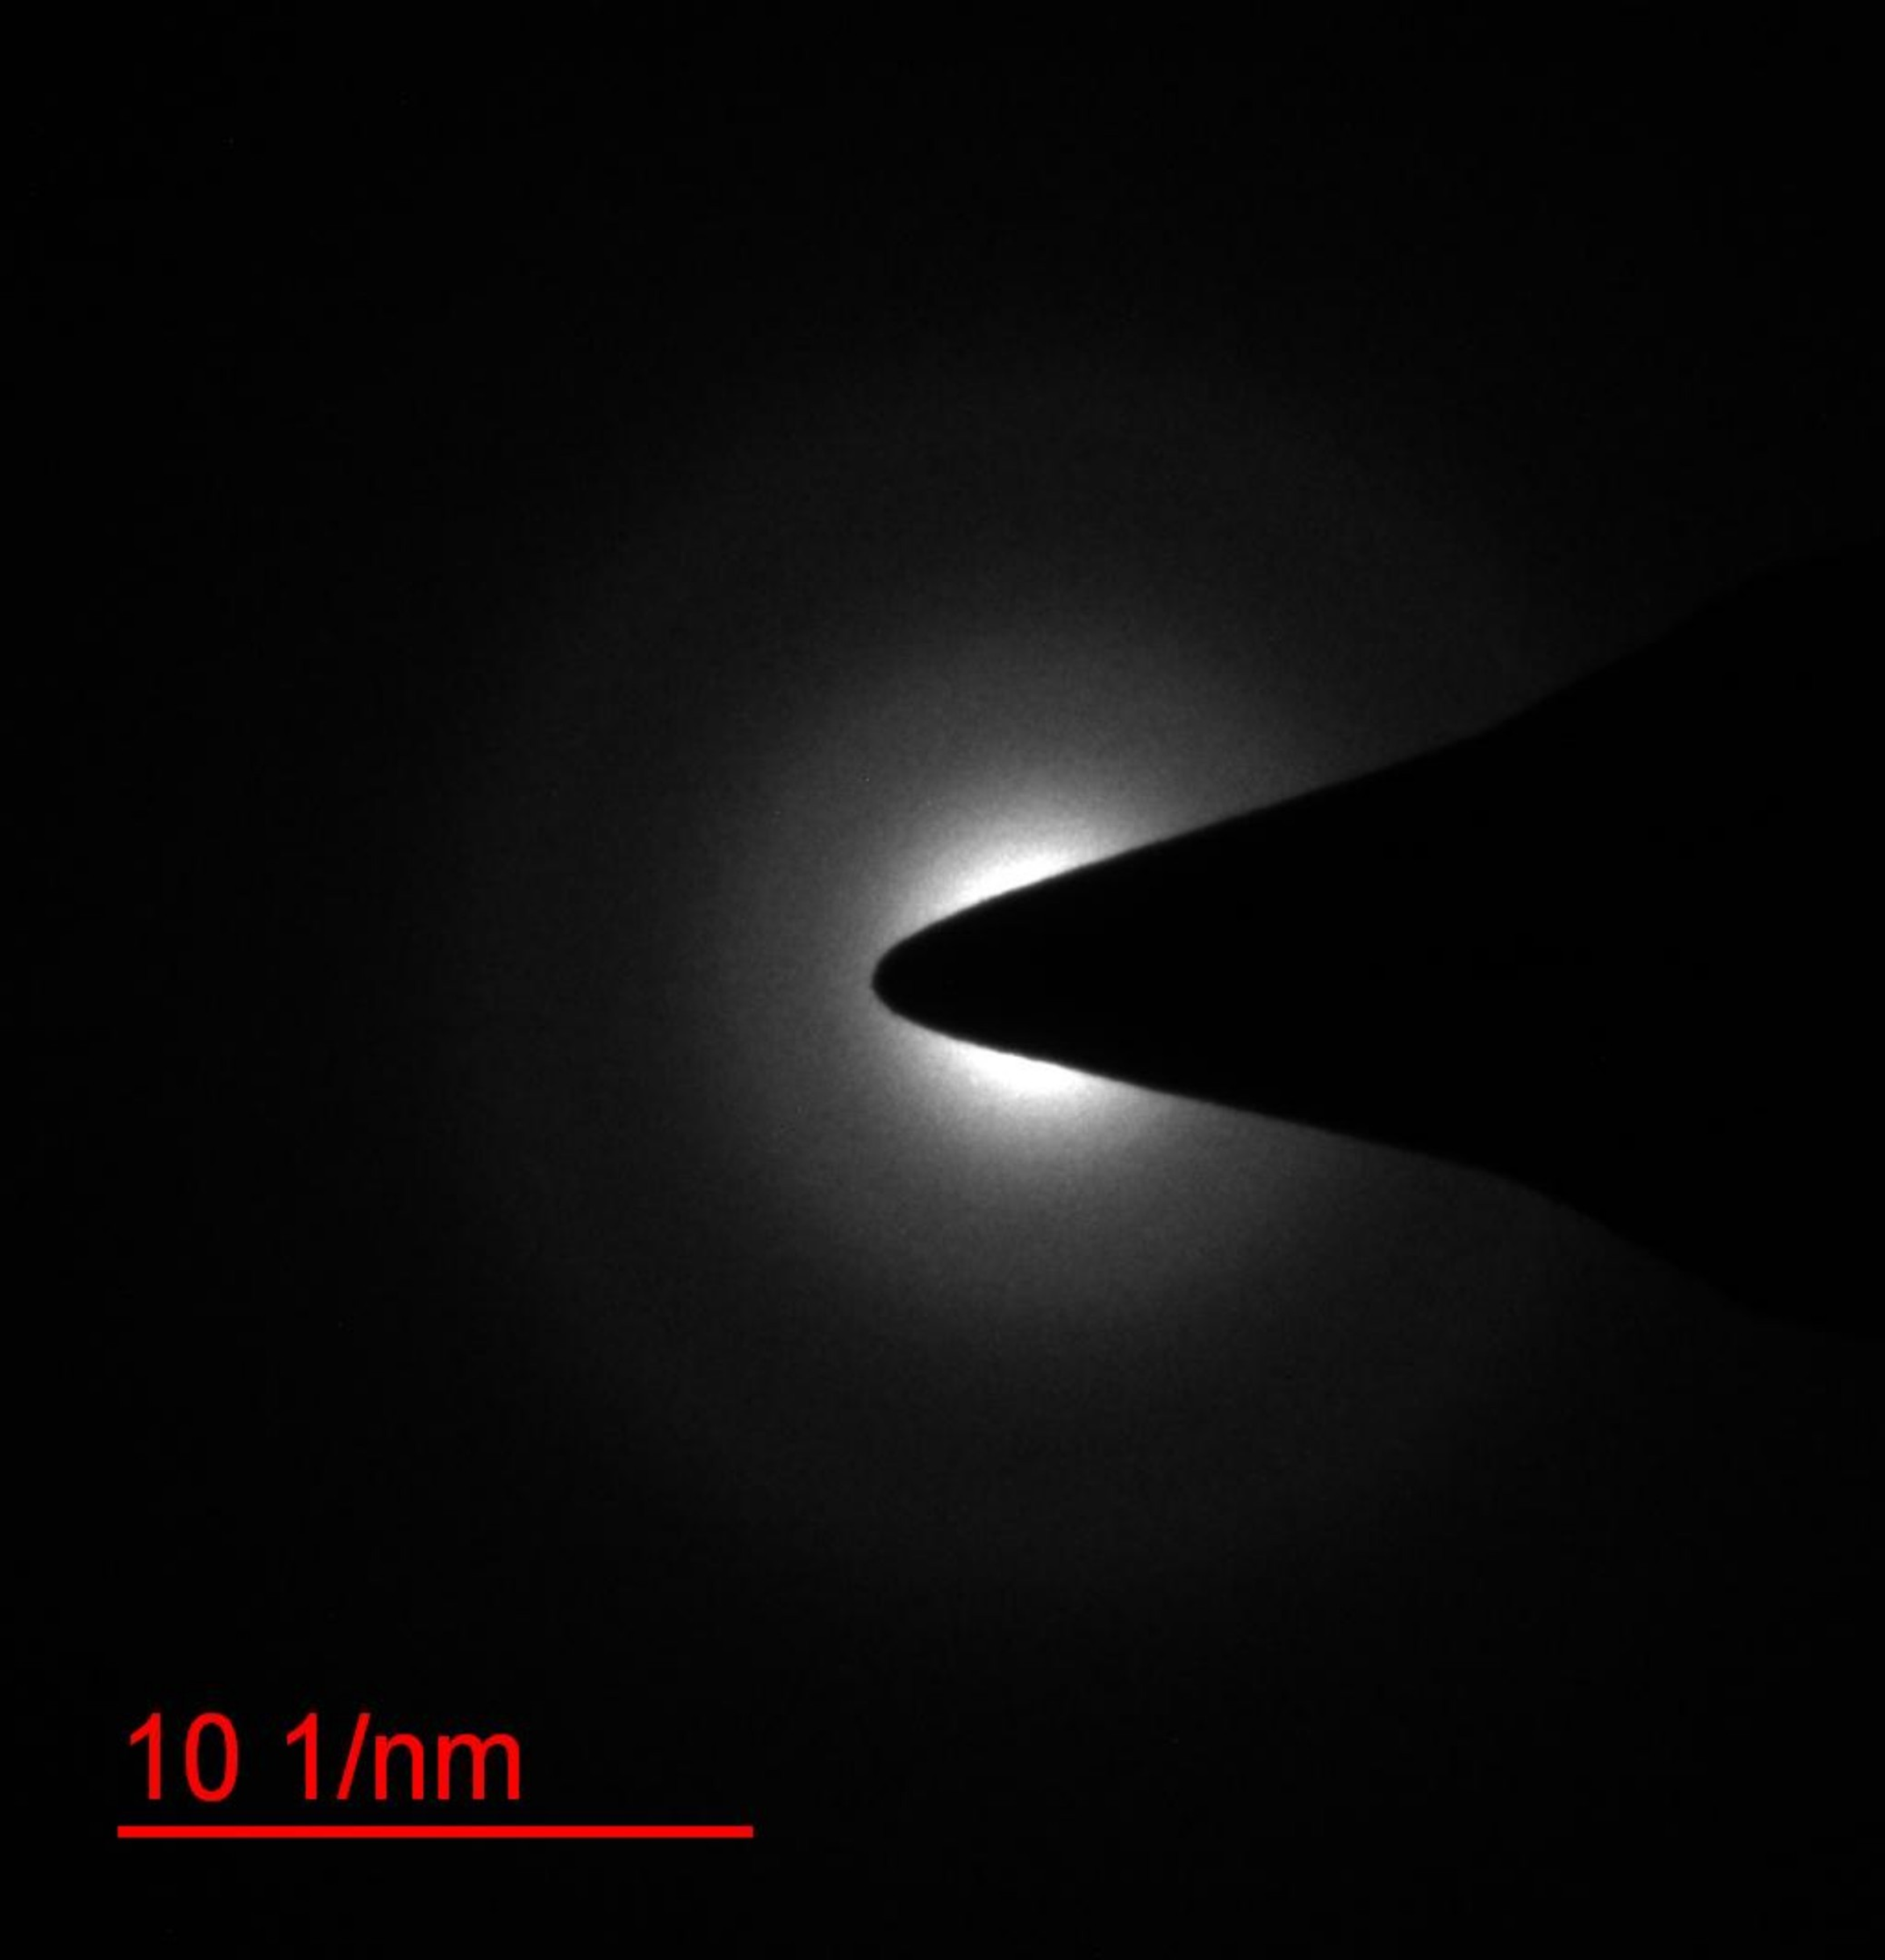
\includegraphics[width=0.55\textwidth]{appendix_figures_p1/Picture1.png}
	\caption[Fig.~SA1: SAED pattern of cross-linked pNAG nanoparticles]{\textbf{Fig.~SA1:}
		Selected area electron diffraction (SAED) pattern of cross-linked
		poly-N-acryloyl glycine (pNAG) nanoparticles.}
	\label{fig:sa1_saed}
\end{figure}

\begin{figure}[htbp]
	\centering
	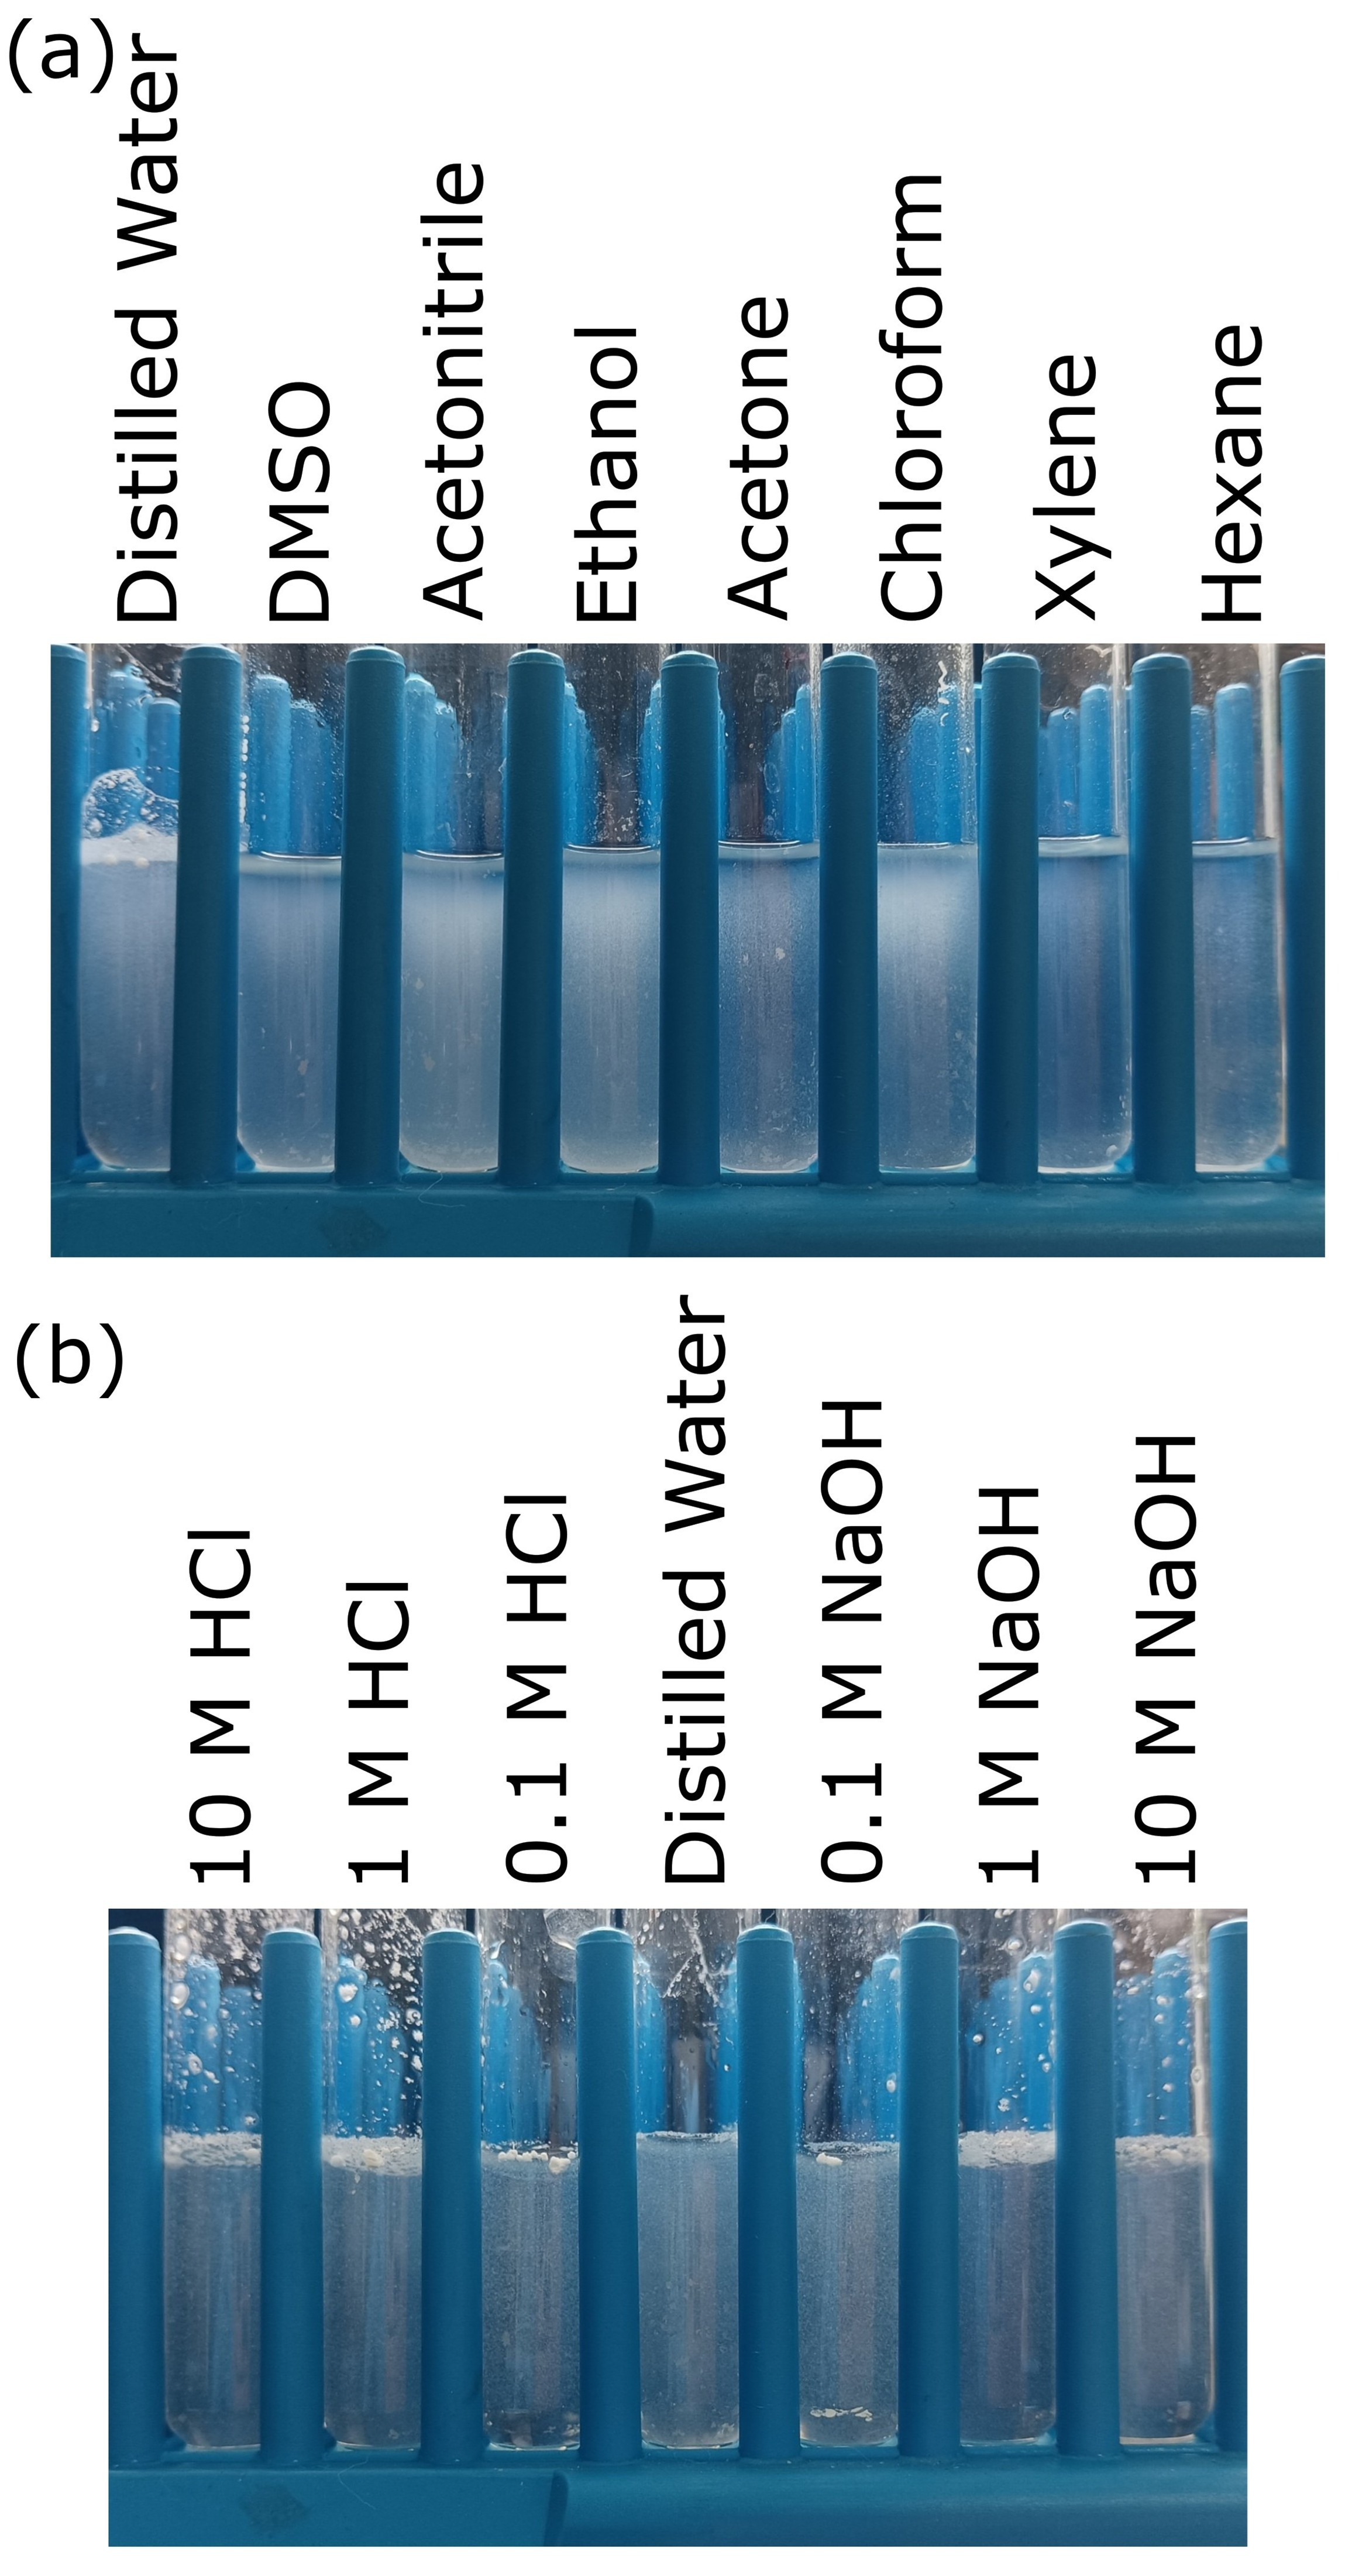
\includegraphics[width=0.85\textwidth]{appendix_figures_p1/Picture2.jpg}
	\caption[Fig.~SA2: Solubility of pNAG nanoparticles]{\textbf{Fig.~SA2:}
		Solubility of pNAG nanoparticles.
		\textbf{(a)}~Solubility in different solvents: distilled water, dimethyl
		sulfoxide (DMSO), acetonitrile, ethanol, acetone, chloroform, xylene, and hexane.
		\textbf{(b)}~Solubility at different molar concentrations of HCl and NaOH.}
	\label{fig:sa2_solubility}
\end{figure}

\begin{figure}[htbp]
	\centering
	\includegraphics[width=0.85\textwidth]{appendix_figures_p1/Picture3.png}
	\caption[Fig.~SA3: Nerve conduction velocity of ventral caudal nerve in rats]{\textbf{Fig.~SA3:}
		Nerve conduction velocity (NCV) of the ventral caudal nerve of rats with a
		stimulation-to-recording distance of 10\,cm.
		\textbf{(a)}~Diabetic treated rat.
		\textbf{(b)}~Non-diabetic normal rat.
		\textbf{(c)}~Diabetic untreated rat.}
	\label{fig:sa3_ncv}
\end{figure}

\begin{figure}[htbp]
	\centering
	\includegraphics[width=\textwidth]{appendix_figures_p1/Picture4.png}
	\caption[Fig.~SA4: ECG of rats -- Lead I, II, III on day 0]{\textbf{Fig.~SA4:}
		Electrocardiogram (ECG) of rats recorded for lead I, lead II, and lead III
		on \textbf{day 0} of treatment.
		\textbf{(a)}~Normal rat.
		\textbf{(b)}~Diabetic treated rat.
		\textbf{(c)}~Diabetic untreated rat.}
	\label{fig:sa4_ecg_day0}
\end{figure}

\begin{figure}[htbp]
	\centering
	\includegraphics[width=\textwidth]{appendix_figures_p1/Picture5.png}
	\caption[Fig.~SA5: ECG of rats -- Lead I, II, III on day 15]{\textbf{Fig.~SA5:}
		Electrocardiogram (ECG) of rats recorded for lead I, lead II, and lead III
		on \textbf{day 15} of treatment.
		\textbf{(a)}~Normal rat.
		\textbf{(b)}~Diabetic treated rat.
		\textbf{(c)}~Diabetic untreated rat.}
	\label{fig:sa5_ecg_day15}
\end{figure}

\begin{figure}[htbp]
	\centering
	\includegraphics[width=\textwidth]{appendix_figures_p1/Picture6.png}
	\caption[Fig.~SA6: Long-duration ECG traces across groups and time points]{\textbf{Fig.~SA6:}
		Electrocardiogram of rats recorded continuously for at least 5\,min,
		illustrating ECG variability across treatment groups and time points.
		\textbf{(a)}~Normal rat, day 0.
		\textbf{(b)}~Normal rat, day 7.
		\textbf{(c)}~Normal rat, day 15.
		\textbf{(d)}~Diabetic treated rat, day 0.
		\textbf{(e)}~Diabetic treated rat, day 7.
		\textbf{(f)}~Diabetic treated rat, day 15.
		\textbf{(g)}~Diabetic untreated rat, day 0.
		\textbf{(h)}~Diabetic untreated rat, day 7.
		\textbf{(i)}~Diabetic untreated rat, day 15.}
	\label{fig:sa6_ecg_long}
\end{figure}

\begin{figure}[htbp]
	\centering
	\includegraphics[width=\textwidth]{appendix_figures_p1/Picture7.png}
	\caption[Fig.~SA7: HRV analysis -- time-domain parameters]{\textbf{Fig.~SA7:}
		Heart rate variability (HRV) analysis of rat ECG (time-domain parameters).
		\textbf{(a)}~R--R interval of untreated diabetic rat.
		\textbf{(b)}~R--R interval of treated diabetic rat.
		\textbf{(c)}~R--R interval of normal non-diabetic rat.
		\textbf{(d)}~Radar plot of mean HRV, SDNN, and RMSSD across all groups.
		\textbf{(e)}~Radar plot of pNN20 and pNN50 across all groups.}
	\label{fig:sa7_hrv_time}
\end{figure}

\begin{figure}[htbp]
	\centering
	\includegraphics[width=0.75\textwidth]{appendix_figures_p1/Picture8.png}
	\caption[Fig.~SA8: HRV analysis -- frequency-domain parameters]{\textbf{Fig.~SA8:}
		Heart rate variability (HRV) analysis of rat ECG (frequency-domain parameters).
		\textbf{(a)}~Radar plot of low-frequency (LF) and high-frequency (HF) power
		across all groups.
		\textbf{(b)}~Radar plot of the LF/HF ratio across all groups.}
	\label{fig:sa8_hrv_freq}
\end{figure}

\begin{figure}[htbp]
	\centering
	\includegraphics[width=0.75\textwidth]{appendix_figures_p1/Picture9.png}
	\caption[Fig.~SA9: HRV analysis -- nonlinear parameters]{\textbf{Fig.~SA9:}
		Heart rate variability (HRV) analysis of rat ECG (nonlinear parameters).
		\textbf{(a)}~Radar plot of Poincar\'{e} plot indices SD1 and SD2 across all
		groups.
		\textbf{(b)}~Radar plot of sample entropy and Lempel--Ziv complexity (LZC)
		across all groups.}
	\label{fig:sa9_hrv_nonlin}
\end{figure}

